\documentclass{article}

%% Page Margins %%
\usepackage{geometry}
\geometry{
    top = 0.75in,
    bottom = 0.75in,
    right = 0.75in,
    left = 0.75in,
}

\usepackage{amsmath}
\usepackage{graphicx}
\usepackage{tikz}
\usepackage{parskip}

\title{Lab 1: Building Circuits}

% TODO: Enter your name
\author{Frederick Meneses}

\begin{document}
\maketitle

The preparation exercises for this lab involve the design of digital circuits using AND, OR and NOT gates that implement a specified behaviour.
However, to make this work in the real world, these gates are built into the 7400-series chips as described in the lab handout.
So your circuit diagrams also need to specify how many of these chips your design needs, and how the pins on the chips you use correspond to the pins on your circuit diagram.
Luckily, Logisim Evolution includes this information.

Your task is to design the circuits in Parts I and II using \textbf{only 74LS04 (NOT), 74LS08 (AND) and 74LS32 (OR) chips}.
In Logisim Evolution, these correspond to 7404, 7408, and 7432, respectively, under \verb|TTL|.
Choose the actual pin numbers of the chips that you will use when you build your circuit and show them on your circuit diagram;
this makes the construction of your physical circuit easier.

For each logic function, show all of the steps required to go from the specification to the final circuit.
This includes:

\begin{itemize}
\item Deriving a truth table
\item Drawing a schematic of the final circuit
\item Assigning names to input and output wires on your schematic
\item Deriving a simplified logic expression, when applicable
\end{itemize}

You can and should use Logisim Evolution to help you.
The \verb|Poke| tool helps you debug your schematic.
The \verb|Analyze Circuit| option helps you compare your own truth table derivation with what Logisim infers from your schematic.
When your schematic is complete, use Logisim's \verb|File -> Export Image| so that you can include it in your report.
You can also export the contents of \verb|Analyze Circuit| into Latex, which includes the truth table.
An example is demonstrated on the next page.
You can use it as a guide for Parts I and II.

\newpage
\section*{Example}

Consider the Boolean function: $f = ab + (c + b)$.
Perform the following steps.

\begin{enumerate}

\item Write out the truth table for the function.

\begin{center}
\begin{tabular}{ccc|c}
$a$&$b$&$c$&$f$\\
\hline
$0$&$0$&$0$&$0$\\
$0$&$0$&$1$&$1$\\
$0$&$1$&$0$&$1$\\
$0$&$1$&$1$&$1$\\
$1$&$0$&$0$&$0$\\
$1$&$0$&$1$&$1$\\
$1$&$1$&$0$&$1$\\
$1$&$1$&$1$&$1$\\
\end{tabular}
\end{center}

\item Draw a schematic that implements the function using only the allowed chips.

\begin{figure}[h!]
    \centering
    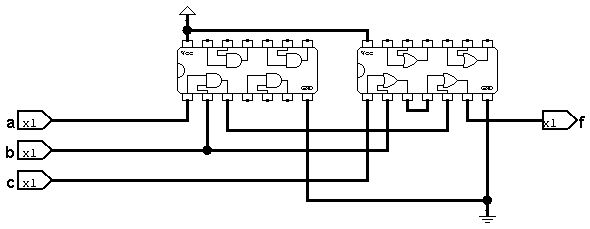
\includegraphics[width=0.5\textwidth]{example.png}
    \caption{A schematic of the example function.}
    \label{f:example}
\end{figure}

\item Is there a cheaper implementation for your design?
    Explain why or why not.
    If there is, include a schematic and discuss how much cheaper it is.

Yes.
We start by minimizing the original equation.

\begin{align*}
    f   &= ab + (c + b)\\
        &= ab + c + b\\
        &= ab + b + c\\
        &= b + c \tag{Covering}\\
\end{align*}

The schematic for the minimized equation would only require a single 74LS32 chip (Figure~\ref{f:example_reduced}), which is 1 chip (and 2 gates) less than the original schematic (Figure~\ref{f:example}).

\begin{figure}[!ht]
    \centering
    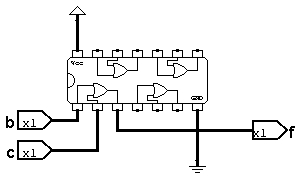
\includegraphics[width=0.3\textwidth]{example_reduced.png}
    \caption{A schematic of the example function, with reduced cost.}
    \label{f:example_reduced}
\end{figure}
\end{enumerate}

\newpage
\section*{Part I}

Consider the Boolean function: $f = x\overline{s}+ys$ (a 2-to-1 multiplexer).
Perform the following steps.

\begin{enumerate}

\item Write out the truth table for the function.
% TODO
\begin{center}
\begin{tabular}{ccc|c}
$x$&$y$&$s$&$f$\\
\hline
$0$&$0$&$0$&$0$\\
$0$&$0$&$1$&$0$\\
$0$&$1$&$0$&$0$\\
$0$&$1$&$1$&$1$\\
$1$&$0$&$0$&$1$\\
$1$&$0$&$1$&$0$\\
$1$&$1$&$0$&$1$\\
$1$&$1$&$1$&$1$\\
\end{tabular}
\end{center}
\item Draw a schematic that implements the function using only the allowed chips.
% TODO

\begin{figure}[!ht]
    \centering
    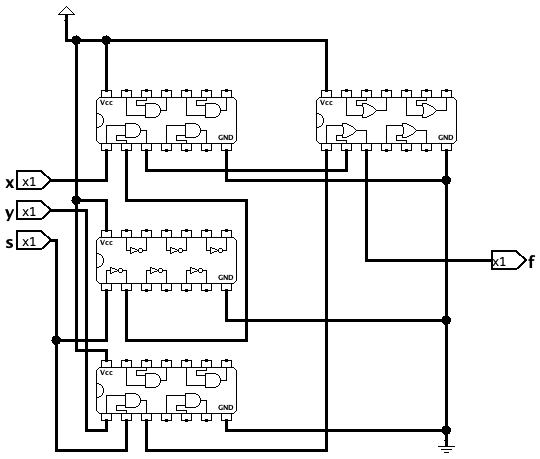
\includegraphics[width=0.7\textwidth]{lab1_part1.png}
    \caption{A schematic of a 2-to-1 multiplexer.}
    \label{f:lab1_part1}
\end{figure}

\item Is there a cheaper implementation for your design, assuming you are still limited to using the same three chip types?
    Explain why or why not.
    If there is, include a schematic and discuss how much cheaper it is.
    % TODO
Yes. There are two methods to make this implementation cheaper.

Notice, we do not need separate chips to perform the same operation.

\begin{figure}[!ht]
    \centering
    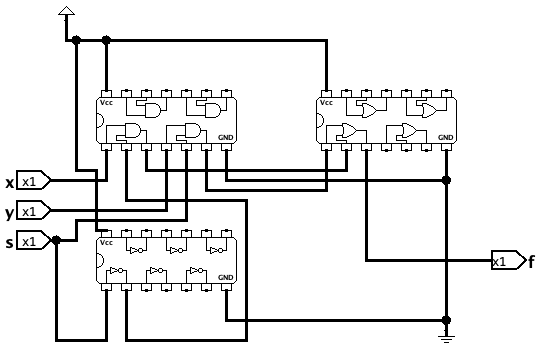
\includegraphics[width=0.7\textwidth]{lab1_part1_cheaper.png}
    \caption{A schematic of the 2-to-1 multiplexer function, with reduced cost.}
    \label{f:lab1_part1_cheaper}
\end{figure}
\newpage

The schematic for this equation would require a 74LS32 chip, a 74LS04 chip, and a 74LS08 chip.(Figure~\ref{f:lab1_part1_cheaper}), which is 1 chip less than the original schematic (Figure~\ref{f:lab1_part1}).

Now we minimize the original equation.

\begin{align*}
    f   &= x\overline{s}+ys\\
        &= \overline{\overline{x} + s}+\overline{\overline{y} + \overline{s}} \tag{De Morgan's Laws}\\
\end{align*}

\begin{figure}[!ht]
    \centering
    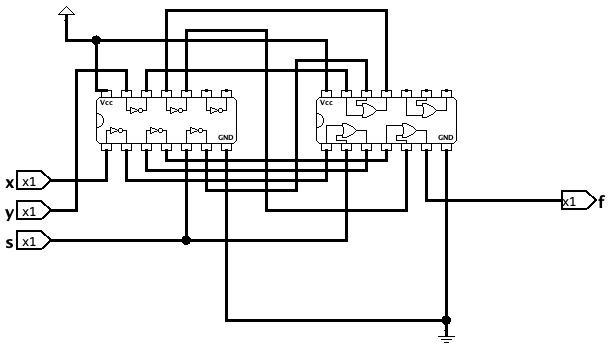
\includegraphics[width=0.7\textwidth]{lab1_part1_cheapest.png}
    \caption{A schematic of the 2-to-1 multiplexer function, with reduced cost.}
    \label{f:lab1_part1_cheapest}
\end{figure}
The schematic for this minimized equation would require a 74LS32 chip, a 74LS04 chip (Figure~\ref{f:lab1_part1_cheapest}), which is 2 chips less than the original schematic (Figure~\ref{f:lab1_part1}) although, it requires more wires.
\end{enumerate}

\newpage
\section*{Part II}

Consider the Boolean function: $f = \overline{a + b} + c\overline{b}$.
Perform the following steps.

\begin{enumerate}

\item Write out the truth table for the function.
% TODO
\begin{center}
\begin{tabular}{ccc|c}
$x$&$y$&$s$&$f$\\
\hline
$0$&$0$&$0$&$1$\\
$0$&$0$&$1$&$1$\\
$0$&$1$&$0$&$0$\\
$0$&$1$&$1$&$0$\\
$1$&$0$&$0$&$0$\\
$1$&$0$&$1$&$1$\\
$1$&$1$&$0$&$0$\\
$1$&$1$&$1$&$0$\\
\end{tabular}
\end{center}
\item Draw a schematic that implements the function using only the allowed chips.
% TODO

\begin{figure}[!ht]
    \centering
    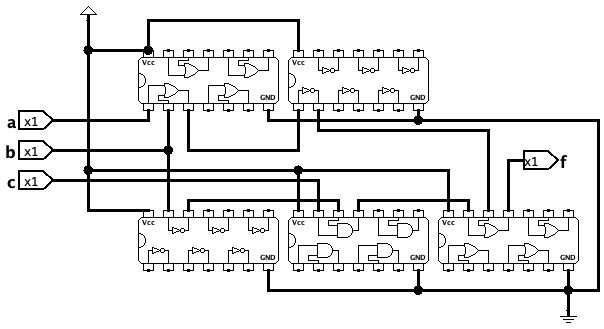
\includegraphics[width=0.7\textwidth]{lab1_part2.png}
    \caption{A schematic of the function from Part II.}
    \label{f:lab1_part2}
\end{figure}

\item Is there a cheaper implementation for your design, assuming you are still limited to using the same three chip types?
    Explain why or why not.
    If there is, include a schematic and discuss how much cheaper it is.
    % TODO
    A cheaper implementation for my design with the given restrictions uses the following minimized equation:
    
    \begin{align*}
    f   &= \overline{a + b} + c\overline{b}\\
        &= \overline{a + b} + \overline{\overline{c} + b} \tag{De Morgan's Laws}\\
\end{align*}

\begin{figure}[!ht]
    \centering
    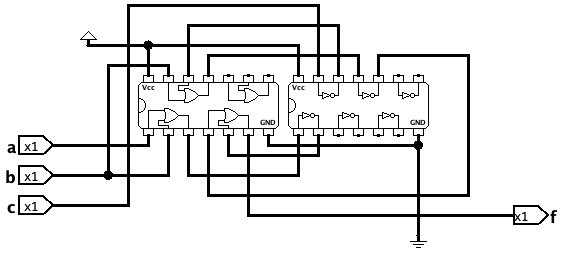
\includegraphics[width=0.7\textwidth]{lab1_part2_cheaper.png}
    \caption{A schematic of the function from Part II, with reduced cost.}
    \label{f:lab1_part2_cheaper}
\end{figure}
The schematic for this minimized equation would require a 74LS32 chip, a 74LS04 chip (Figure~\ref{f:lab1_part2_cheaper}), which is 3 chips less than the original schematic (Figure~\ref{f:lab1_part2}).

\end{enumerate}
\newpage
\section*{Part III}

Draw a schematic of the 2-to-1 mux, but instead of using the \verb|TTL| chips, use the NOT, AND, and OR gates directly (i.e., under \verb|Gates|).

\begin{figure}[!ht]
    \centering
    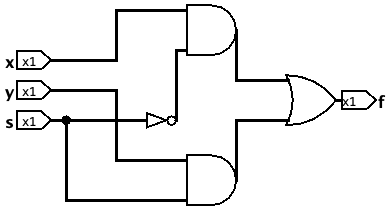
\includegraphics[width=0.5\textwidth]{lab1_part3.png}
    \caption{A schematic of the 2-to-1 multiplexer from Part III.}
    \label{f:lab1_part3}
\end{figure}

\end{document}
